\section*{Scattered photon energy}
To study the angular dependence of the scattered $\gamma$ a coincidence between the three detectors was selected as trigger of the system. The coincidence between Tagger and Scatterer ensures the detection of the  two collinear 511~keV $\gamma$ from the $^{22}$Na source, then the triple coincidence with the Detector allows to select the Compton scattered $\gamma$ at chosen angle. The data collection was performed over six different angles from 0$^\circ$ to 90$^\circ$, the last one~(90$^\circ$) through a night run because of the lower rate~(see Tab.~\ref{Tab:Rates}). 
\begin{table}[H]
	\centering
	\begin{tabular}{cc}
		\toprule
		\toprule
		 Angle & Rate[Hz] \\
		\midrule
		   0$^\circ$ & 7.3 \\
		20$^\circ$ & 6.8\\
	    40$^\circ$ & 4.6\\
	    60$^\circ$ & 3.4\\
	    70$^\circ$ & 3.1\\
	    90$^\circ$ & 2.3\\
		\bottomrule
		\bottomrule
	\end{tabular}
	\caption{Triple coincidence rates measured in a 30~s time interval.}
	\label{Tab:Rates}
\end{table}

The energy of recoil electrons and scattered $\gamma$ measured by the Scatterer and Detector respectively, as a function of scattering angle, is presented in Fig.~\ref{Fig:Scattering_angles}.

\begin{figure}[h!]
	\centering
	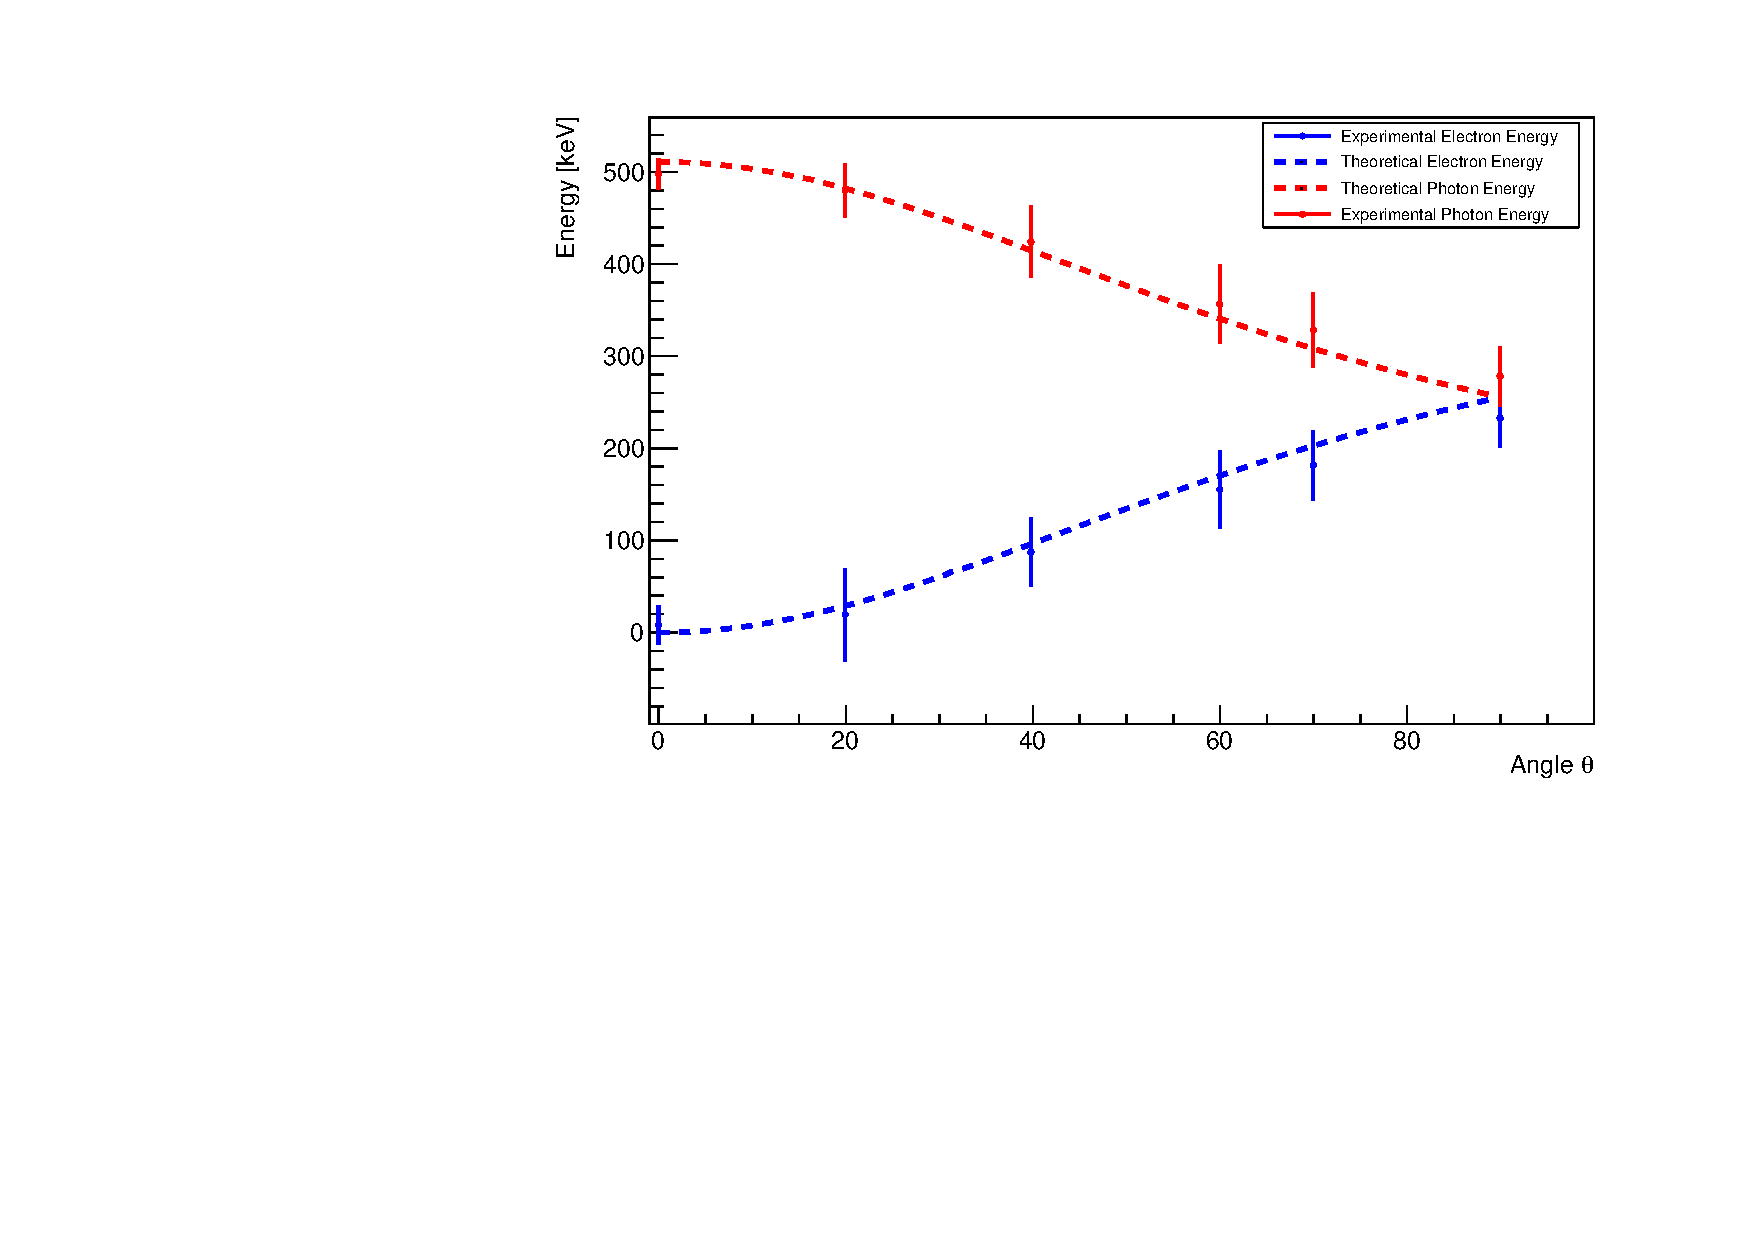
\includegraphics[width=\textwidth]{Angular_photon_energy}
	\caption{Energies of the scattered $\gamma$ and recoil electrons at different scattering angles.}
	\label{Fig:Scattering_angles}
\end{figure}